\documentclass{article}
\usepackage{graphicx}

\begin{document}

\title{Thesis Proposal}
\author{Adam Yedidia}

\maketitle

\begin{abstract}
For my thesis, I propose to write a general-purpose compiler from a programming language of my design to a single-tape, two-symbol Turing machine with as few states as possible. Once this is complete, I propose to write a program in my language that will verify the consistency of Zermelo-Fraenkel set theory (or ZFC), and compile that program down into a Turing machine description. In so doing, I will have created a description for a Turing machine whose behavior cannot be predicted by ZFC. This is true by inspection, because since a logic system cannot prove its own consistency, a logic system cannot prove whether or not a Turing machine that verifies its consistency accepts or rejects.
\end{abstract}

\section{Definitions}

For the purposes of this proposal, a \emph{single-tape, two-symbol Turing machine} (STTSTM) is a theoretical finite-state machine with infinite memory that can only be accessed in a specific way. More specifically, a Turing machine's memory lies on a one-dimensional \emph{tape} which extends infinitely in both directions. The tape is divided into discrete \emph{locations}, each of which can hold one of two symbols (a 0 or a 1). \\

I will speak of the Turing machine as having a \emph{head}, which occupies a specific location somewhere on the tape. At each step of the Turing machine's evaluation, the machine may read the symbol that is at the head's location, and then based on the symbol read and on the state the Turing machine currently occupies, the machine can write a new symbol at the head's current location, may move the head right or left or keep it where it is, and may enter a new state. The Turing machine may also enter one of two special states, called the \emph{accept} and \emph{reject} states, which halt the Turing machine's computation. A Turing machine that enters an accept state is said to have \emph{accepted}; a Turing machine that enters a reject state is said to have \emph{rejected}. \\

A \emph{multi-tape, multi-symbol Turing machine} (MTMSTM) differs only from the previously-described machine in the number of infinite tapes that the machine uses to write on, and in the number of separate symbols that can be read or written. Unlike an STTSTM, an MTMSTM has a finite alphabet of symbols to draw from, whose size need not be two. Moreover, an MTMSTM has a finite number of tapes, and a head on each one that can be moved. Each state that an MTMSTM has available to it specifies along with it a tape which can be read or written from in that state. \\

Note that unlike my definition of STTSTMs, my definition of MTMSTMs is not the unique definition used in the literature. Plenty of other definitions exist, including ones that involve reading from or writing to all the tapes of the Turing machine at once. To create a MTMSTM is not my ultimate goal; rather, my ultimate goal is to create an STTSTM from a written program, with the creation of MTMSTM being a useful intermediate step. Therefore, I defined the MTMSTM in order to make my later task of converting it to an efficient STTSTM as easy as possible.

\section{Overview}

The figure below provides a visual overview of how I've divided the task of generating a Turing machine description that simulates a specific TURD program.

\begin{figure} 
\begin{center} 
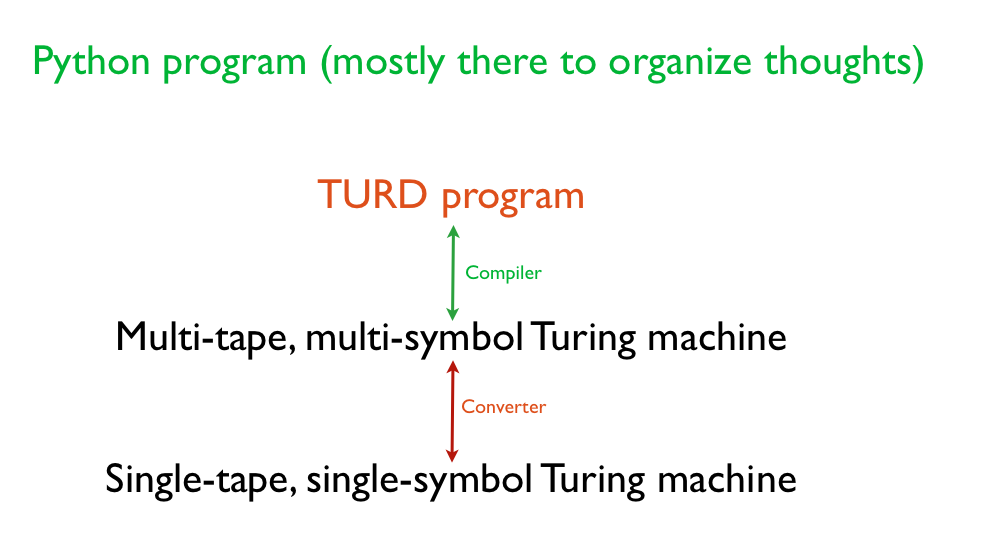
\includegraphics[height=3in,width=5in,angle=0]{overview.png} 
\caption{A visual overview of the machinery used to ultimately create the desired Turing machine description. Green indicates something that I have implemented already; red indicates something that has not yet been implemented. Black indicates something that does not require appreciable effort (for example, creating a custom multi-tape, multi-symbol Turing machine is trivial given an appropriate TURD program and a compiler).\label{fig:Stupendous}} 
\end{center} 
\end{figure}

\section{TURD}

Initially, I set out to write a general compiler from Python (the programming language I am most familiar with) to an MTMSTM. This quickly proved very impractical, because Python is a very powerful language with many options. To explain to the compiler how to convert each of the many Python commands to an MTMSTM description would take much too long and be way too complicated for the scope of this project. To make things easier, I decided to create my own programming language. I called it TURD (TURing machine Descriptor). For simplicity of writing the compiler, I created TURD not to be a user-friendly language but to have as few distinct commands as possible. The commands that I created for it are: \\ \\
\texttt{var x}: Declares variable x. \\
\texttt{assign x to [expr]}: Assigns to variable x the value given by the expression \texttt{[expr]}. Expression \texttt{[expr]} is an expression of one or two variables, using one of a short list of operations, including the standard arithmetic operations (\texttt{+}, \texttt{-}, \texttt{/}, \texttt{*}), the standard boolean operations (\texttt{and}, \texttt{or}, \texttt{not}) and a few list operations (\texttt{append}, \texttt{index}). \\
\texttt{label L}: Gives this line of code the label L. \\
\texttt{goto L}: The new line of code being run becomes the line of code with label L. \\
\texttt{print x}: If I'm testing my code by evaluating it in Python, print the value of variable x. If this program is being compiled down to a Turing machine description, ignore it. \\
\texttt{accept}: The machine accepts. \\
\texttt{reject}: The machine rejects. \\

Note that TURD is Turing-complete. While it is substantially less convenient than a normal language like Python, it can theoretically do anything that can be done in Python. Note, also, that for convenience of writing sophisticated programs in TURD, I made the language support arbitrarily-nested lists (which are very natural to represent on a Turing machine tape). \\

In the design of TURD, I have two goals that pull me in opposite directions. The first is that I want the program that converts TURD programs to MTMSTM descriptions to be easy to write. This goal makes me want to make TURD as parsimonious and weak a language as possible, so that there aren't very many cases to write. My second goal, however, is that I want to write a program in TURD that will verify the consistency of ZFC. This goal makes me want to make TURD as complicated and powerful a language as possible, so that I can write whatever program I want with minimal effort. At the moment, TURD is a very weak language, and I've written the part of the compiler that converts a computer program written in TURD to a description for an MTMSTM. I expect that as I find myself trying to write the program that I actually wanted to write in TURD, I will start adding features to TURD. I expect the language to evolve, and I think it's very likely that by the conclusion of the project it'll have many more commands available.

\section{Conversion of STTSTMs to MTMSTMs}
Proving that a general-purpose converter from STTSTMs to MTMSTMs could be made is a common exercise in Theory of Computation classes, but the actual implementation of such a converter is far from easy. This is a part of my compiler that I haven't written yet. \\

Before I can discuss how I'm going to convert my MTMSTM to an STTSTM, I have to describe how my MTMSTM is designed. In my MTMSTM, I make use of one of six types of symbols: \texttt{1}, \texttt{\_}, \texttt{[}, \texttt{,}, \texttt{]}, \texttt{E}. A variable's value is represented in unary. Each variable has its own tape. Each of the symbols has some meaning, which I did my best to keep consistent for my own sanity if for nothing else. \\

\texttt{1} has as its meaning a single unit in unary. \texttt{\_} is the empty symbol, which fills the tape at the start of execution. \texttt{[} and \texttt{]} are begin and end list, which have the same meanings that they would in Python, for example. \texttt{,} means ``next item in the list.'' \texttt{E} means ``end of value''  \\

As an example, let us suppose that at a certain point in a compiled TURD program's execution, there are four variables, that have the values \texttt{5}, \texttt{[2, 4]}, \texttt{0}, and \texttt{[[3,4], 5, []]}. Then, the MTMSTM that the TURD program would compile down to would at that point in its execution have four tapes, with the first tape reading \dots\texttt{\_\_\_\_11111E\_\_\_\_}\dots, the second tape reading \dots\texttt{\_\_\_\_[11,1111]E\_\_\_\_}\dots, the third tape reading \dots\texttt{\_\_\_\_E\_\_\_\_}\dots, and the fourth tape reading \dots\texttt{\_\_\_\_[[111,1111],11111,[]]E\_\_\_\_}\dots. \\

When converting the STTSTM to an MTMSTM, there are two separate challenges that must be tackled. The first is that these four tapes' contents must all fit on a single tape. The second is that this larger alphabet needs to be condensed down to a two-symbol alphabet. I'll discuss the first challenge now.

\subsection{Reduction to one tape}

After we throw off the abstraction of the MTMSTM, there are a few more concerns that we need to deal with that will necessitate the introduction of a few new symbols. In particular, now that we no longer have multiple heads, but wish to keep the abstraction of having multiple heads, we need to write the location of each of the ``fake heads'' down on the tape somewhere. Each of the different variables we're tracking needs its own associated head location. Moreover, we need to differentiate between the beginning of one variable's value and the next variable's head location, and one variable's head location and that same variable's value. We also need each variable to have a name that the tape head can identify while scanning the tape, so that we can go to the right variable and change it appropriately.  \\

In addition to this concern, we need to make some symbol marking the last variable's value. And finally, we need to have some mechanism for ``expanding'' the amount of room devoted to each variable if that variable becomes large, since unlike in the old situation, we don't have an infinite amount of space devoted to each individual variable, only to the collection of variables. Naturally, with that requirement comes the symmetric requirement that we have a mechanism for expanding the amount of room devoted to showing the tape head's index.\\

In order to address these concerns, I use an expanded set of symbols. The new set of symbols that I use are \texttt{1}, texttt{\_}, \texttt{[}, \texttt{]}, \texttt{,}, \texttt{N}, \texttt{H}, \texttt{E}, and \texttt{F}. \texttt{1} is a unit in a unary number, \texttt{\_} is the empty symbol as before, and \texttt{[}, \texttt{,}, and \texttt{]} are the symbols associated with lists. Now, however, we have a few more symbols: \texttt{N} is the symbol that means ``end the value that tells you which variable this value represents, and begin the value that tells you the location of the tape head,'' \texttt{H} is the symbol that means ``end the value that tells you the location of the tape head and begin the value that tells you the variable's value,'' \texttt{E} is the symbol that means ``end the value that tells you the variable's value,'' and \texttt{F} is the symbol that means ``this is the end of the last variable.'' \\

As before, this design is near-impossible to explain intelligibly without an example. Here's one now! \\

Let's suppose we have our four variables from before. Let's also suppose that our four tape ``heads'' are in positions 1, 5, 1, and 1. (In between lines of code, I will require that tape heads return to position 1, although that's a discussion to be expanded further upon in the next section). The way this situation might look on the tape would be the following: \\

\dots\texttt{\_\_\_\_N1H11111E1N11111H[11,1111]E11N1HE111N[[111,1111],11111,[]]EF\_\_\_\_}\dots \\

I say ``might'' because I allow flexibility in terms of how space is allocated to each number. When the size of a number increases, I need to take action to push all the symbols to the right; but when the size of a number decreases, I don't want to have to spend effort pulling everything back to the left. Therefore, I allow underscores as ``empty slots.'' To give a more concrete example, the tape might equally well have looked like \\

\dots\texttt{\_\_\_\_N1H\_\_11111E\_\_\_\_\_\_1N\_\_\_11111H[11,1111]E\_\_\_\_11N1HE111N\_\_\_\_\_[[111,1111],11111,[]]E\_\_\_\_\_F\_\_\_\_}\dots \\

and in general, I allow any number of underscores after each letter. Figures 2 and 3 provide a more detailed illustration, with color-coded explanations, in case it isn't clear what symbols correspond to what. \\

\begin{figure} 
\begin{center} 
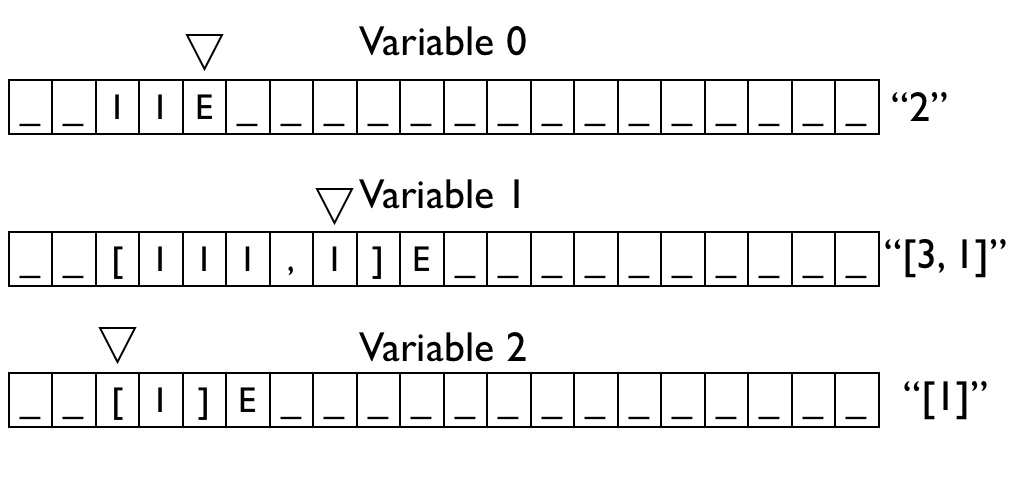
\includegraphics[height=2.5in,width=5in,angle=0]{MTMSTM.png} 
\caption{\small \sl This figure shows what a MTMSTM with three variables might look like. In this example, the three variables have as their values 2, [3,2], and [1], respectively. The upside-down triangles indicate the head locations. .\label{fig:Stupendous}} 
\end{center} 
\end{figure}  

\begin{figure} 
\begin{center} 
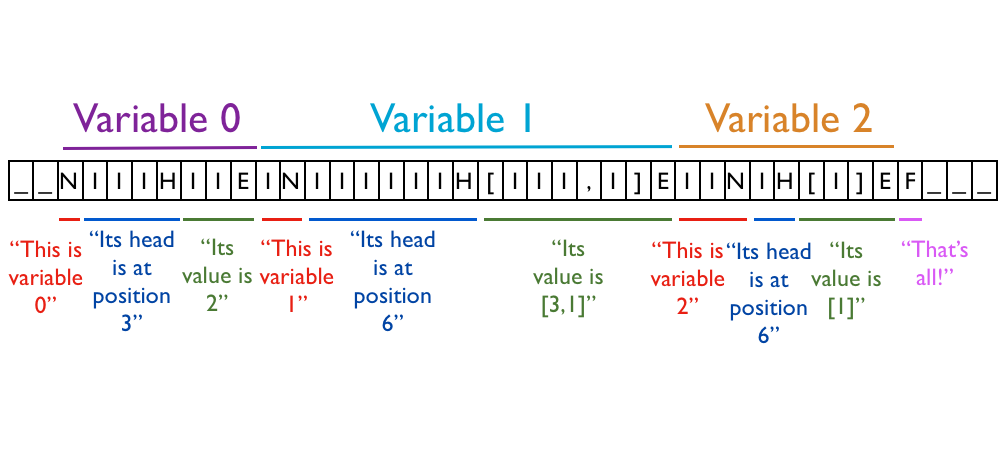
\includegraphics[height=2.5in,width=5in,angle=0]{STTSTM.png} 
\caption{\small \sl This figure shows the same situation, but one level lower: this time, everything must fit on one tape. The verbal color-coded underlines illustrate the English meaning of each of the various sections. Note that as explained earlier, there might be underscores after each letter; in this example, there are none, to preserve space.} 
\end{center} 
\end{figure}  


Addressing the challenge of expanding numbers is tricky, but not fundamentally too different from what we were doing before--it just costs a lot of states. Whenever we do an operation that lengthens a number (such as an append, or an assign) then we need to increase the amount of space allocated to that number by 1 repeatedly, as many times as it takes. The way this happens is simple enough--the head runs over the tape, remembering the last symbol (using nine different states for each of the nine symbols) and writing that symbol onto the next slot on the tape. This needs to happen twice--once to increase the amount of space allocated to the number itself, and once to increase the amount of space allocated to writing down the head's location. (Note that I require that the head's location never go negative, obviating me of the need to be able to write down negative numbers).

\subsection{Reduction to a 2-symbol alphabet}

Finally, we need to take the nine-symbol alphabet described previously and reduce it to a two-symbol alphabet. I do this simply by providing the following mapping of alphabet symbols to binary strings: \\ \\
\texttt{\_} $\leftrightarrow$ \texttt{0000} \\
\texttt{1} $\leftrightarrow$ \texttt{0001} \\
\texttt{[} $\leftrightarrow$ \texttt{0010} \\
\texttt{]} $\leftrightarrow$ \texttt{0011} \\
\texttt{,} $\leftrightarrow$ \texttt{0100} \\
\texttt{N} $\leftrightarrow$ \texttt{0101} \\
\texttt{H} $\leftrightarrow$ \texttt{0110} \\
\texttt{E} $\leftrightarrow$ \texttt{0111} \\ 
\texttt{F} $\leftrightarrow$ \texttt{1000} \\

Thus, the earlier-described string would look like: \\

\dots\texttt{0000000001010001011000010001000100010001011100010101000100010001000100010110001000010001010000010001000100010011011100010001010100010110011100010001}\dots \\

Although at this point the string is well beyond the point of readability, so I won't belabor the issue. But the idea is that now, each former ``read'' and ``write'' will now require nine states to do, since you need nine Turing machine states to track which of the nine possibilities is the one that is happening. Additionally, each time the head needs to move right or left, it will now require four states. \\

It is quite unfortunate that my current alphabet contains nine symbols, which is one more than a power of two. I hope to optimize away one of the symbols, probably by reusing the \texttt{,} symbol in a situation where I know that it can't be what's meant. But this is a job for when I'm working on implementing the converter. \\

It's my hope that I'll be able to automate the process of taking a MTMSTM and converting it to an STTSTM. The hardest part of the conversion is probably going to be the logic for reading and interpreting the information in front of each variable (what the variable's name is, and where the head is currently). Once that's done, systematically converting each read, write, and move into binary-speak should be easily systematized.

\section{Creating the TURD program}

All of this machinery is useless, of course, if I never write the program that I eventually want to turn into a Turing machine description. This program is a program that would check the consistency of ZFC. Naively, the approach one might take to do this would be to take the axioms of ZFC, apply them to themselves in a systematic and exhaustive manner, and if doing this ever yields a contradiction, reject; otherwise, loop forever. This would give us a Turing machine which would co-recognize the consistency of ZFC. \\

This idea is good, but the problem of coming up with a formal language for describing the axioms of ZFC that could be expressed on a Turing machine's tape is a very difficult practical problem. Fortunately, this particular part of the task has been done for me, by one Professor Harvey Friedman, who was kind enough to prove that the following statement's truth or falsehood was equivalent to the consistency of ZFC[1]: \\

\emph{For all $k, n, r \ge 0$, every order invariant graph on $[Q]^{\le k}$ has a free $\{x_1,\dots,x_r,ush(x_1),...,ush(x_r)\}$ of complexity $\le 8knr!$, each
$\{x_1, \dots, x_{(8kni)!}\}$ reducing $[x_1 \cup \dots \cup x_i \cup \{0,\dots,n\}]^{\le k}$.}

In this definition, an ``order invariant graph'' is a graph containing an infinite number of nodes. In particular, it has one node for each finite set of size $k$ of real numbers that exists. Two nodes have an edge between them if and only if the two sets are subject to an ordering specified by the graph. So, for example, a graph might require that an the ordering be (first set, second set, second set, first set), and then sets like \{1, 4\} and \{2, 3\} would have an edge between them, but not sets like \{1, 3\} and \{2, 4\} (because that would require the ordering to be (first set, second set, first set, second set)).  \\

In addition, the ush() function takes as input a set and returns a copy of that set with all non-negative numbers in that set incrememnted by 1. \\ 

A number of complexity at most $c$ refers to a number that can be written as a fraction $a/b$, where $a$ and $b$ are both integers less than or equal to $c$. A set has complexity at most $c$ if all the numbers it contains have complexity at most $c$.

Finally, to take Prof. Friedman's definition fo the term ``reducing'': \\

\emph{A set of vertices $X$ reduces a set of vertices $Y$ if and only if for all $y \in Y$, either $y \in X$ or there is an $x \in X$ such that ($x E y$ and $\max(x) \le \max(y)$)}. \\

Unfortunately, even after one has these definitions and has read the statement enough times to make some sense of it, it's difficult to get an intuition for what the statement is doing. I won't focus on the statement, because although writing a program to check it is the ultimate goal of the project, from the point of view of implementing the project, the most difficult and interesting part is more about the details of how to convert this statement into a Turing machine description. \\

It's possible to check this statement by incrementing $k$, $n$, and $r$ together, and constructing sets based on what they are by enumerating all the numbers of complexity at most $(8knr!)$. Constructing all possible order-invariant graphs simply requires enumerating all the different possible orderings. That's a lot of enumeration, but fortunately minimizing the number of states is all we care about--not efficiency! \\

One note about this statement is that it involves negative numbers and non-integers, neither of which TURD supports (or are easy to adapt to my current Turing machine design). The non-integers aren't much of a worry, since it's easy to just multiply everything out by their denominators. The negative numbers might be annoyance. I haven't yet decided whether it would be more effective to keep a boolean with each number I define, to keep track of whether that number is negative, or whether it would be better to simply add more symbols to support negative unary numbers. \\

\section{Concluding thoughts}

Initially, my idea had been to convert my Python program into C, and from C into Assembly, at which point I would write my compiler from Assembly down to a Turing machine description. This idea, however, was made much less palatable by the fact that Assembly is in fact a very complicated language, with many different features; to implement all of them was a daunting task indeed. Furthermore, the conversion of a Python program to Assembly was not an efficient process; indeed, the number of lines of Assembly code from my Python program checking the above statement numbered in the tens of thousands, so I expect that the ultimate Turing machine that would have resulted would have had a number of states in the tens to hundreds of millions. \\

This is why I invented Turd: to be more or less a version of Assembly with only the operations that were Turing-machine friendly (to make my life easier when writing the compiler) and with support for lists (to make my life easier when writing the program). \\

I expect that as I continue work on this project, my design will evolve substantially, although I expect that the general structure will remain the same. This project has taught me a way of thinking about computation that is very different from the normal one. Whereas normally, optimizing computation means making it as efficient as possible, here, optimizing computation means making it as \emph{parsimonious} as possible. This leads to some weird design decisions--for example, the decision to do everything in unary. It has exposed me to a different kind of logic, and a new set of algorithms to consider. Most of the time, they're easier! For example, unary integer division is far simpler than binary integer division. \\

I believe that this project will continue to teach me about both compilers and about computation theory; I look forward to seeing what I learn in the semester to come.

\section{Bibliography}

Harvey Friedman, “Order Invariant Graphs and Finite Completeness.” June 21, 2014.

\end{document}
